\documentclass[letterpaper, 12pt]{article}
\renewcommand{\refname}{References and Resources}
\usepackage[utf8]{inputenc}
\usepackage{float}
\usepackage{graphicx}
\graphicspath{{pictures/}}
\usepackage{listings}
\usepackage{pgfplots}
\pgfplotsset{compat=1.9}
\usepackage[pdf]{pstricks}
\usepackage{pst-optexp}
\usepackage{hyperref}
\hypersetup{colorlinks=true,linkcolor=blue,filecolor=magenta,urlcolor=cyan}

\setlength{\parskip}{1em}

\title{Modern Physics Laser Scanning Project}
\author{Alvin Lin
  \thanks{with Jion Fairchild and Sachal Malick}}
\date{June 2016}

\begin{document}

\begin{titlepage}
\maketitle
\end{titlepage}

\begin{abstract}
This experiment was conducted in the Modern Physics class of 2016 at Stuyvesant High School. The goal was to build a laser scanner using a laser and a photodiode and find the maximum achievable resolution of the apparatus.
\end{abstract}

\section{Experimental Setup}
\par
In this experiment, we focused a laser onto a piece of paper containing our
scanning sample and read the amount of reflected light using a photometer. The photometer displayed the amount of light it received on a digital display but also conveniently had two banana jacks that outputted a voltage proportional to the amount of light it received. This allowed us to connect an Arduino microcontroller to the photometer to read and store the voltages as we passed the scanning sample beneath the laser. To shift the sample vertically and horizontally during scanning, we 3D printed slides for the sample which we motorized using stepper motors.
\par
In order to maximize the resolution of our image, we wanted the laser beam to be as small and as focused as possible. We spaced three concave lenses in front of the laser to expand the beam, collimate it, and focus it to a point. The scanning sample would be placed at the focal point of the last concave lense. If the laser was focused on a darker point on the sample, it would reflect less light and the photometer would read a lower voltage. Conversely, if the laser was focused on a lighter point, it would reflect more light and the photometer would read a higher voltage.

\begin{pspicture}[](0,0)(14,4)
  \pnodes(2,2){A}(12,2){B}
  \pnodes(10.5,1.5){D}(10.7,2){E}(10.9,2.5){F}
  \begin{optexp}
    \optbox[position=start](A)(B){laser}
    \lens[lensradius=0.75,abspos=1,labeloffset=-1](A)(B){expands beam}
    \lens[lensradius=2.3,abspos=4](A)(B){collimates beam}
    \lens[lensradius=0.75,abspos=8](A)(B){focuses beam}
    \mirror[labeloffset=-0.7](D)(E)(F){sample}
    \drawwidebeam[beamwidth=0.2,linecolor=red]{-}(B)
  \end{optexp}
\end{pspicture}

\par
The Arduino that we used to read in the voltage values from the photometer was also used to simultaneously control the stepper motors moving the sample. For one dimensional scans, we scanned across the sample once and graphed the relative intensities as the laser passed over the sample. For two dimensional scans, we oscillated the sample in one direction while shifting it perpendicular to its direction of oscillation and mapped the relative intensies onto a 2D grid.

\begin{figure}[H]
  \centering
  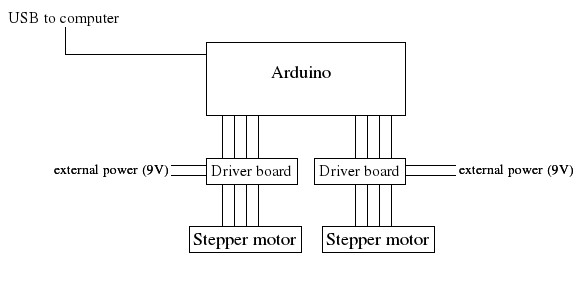
\includegraphics[width=12cm,height=8cm]{setup_diagram}
  \caption{Diagram of Components}
\end{figure}

\newpage

\begin{figure}[H]
  \centering
  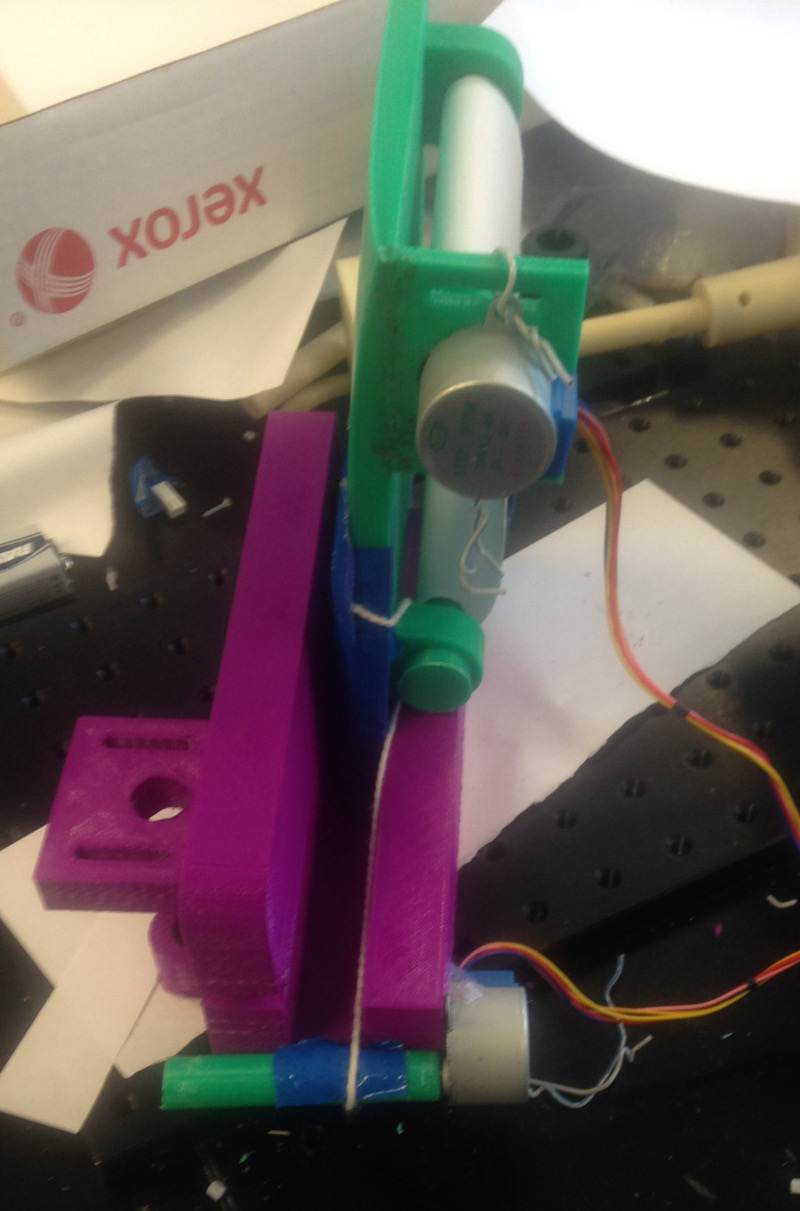
\includegraphics[width=8cm,height=10cm]{setup_picture}
  \caption[caption]{3D printed components\footnotemark}
\end{figure}
\footnotetext{CADs available here:\cite{github}}

\section{Experimental Procedure}
\par
We set up various resolution test targets beneath our scanner and ran our scanner over each target. Based on the stepper motors\footnotemark
\footnotetext{USPRO 28BYJ 5V 4-phase 5-wire stepper motors \cite{amazon}}
and driver boards\footnotemark
\footnotetext{ULN2003 driver board for Arduino \cite{amazon}}
we were using, we approximated what the resolution of our setup would be. Due to the driver board's microstepping, each revolution of the motor took 512 steps. With a 0.5 inch diameter drive axle moving the sample, this means that 1 step of the motor would shift the sample $3.067962\times10^{-3}$ inches. Converting this to $\frac{lines}{mm}$:

$$ 3.067962\times10^{-3}in = 7.79262348\times10^{-2}mm $$
$$ \frac{1\ line}{7.79262348\times10^{-2}mm} \approx 12.83\frac{lines}{mm} $$

\par
This number only holds true if our laser beam is an infinitesimally small point. Since this is not the case, our actual resolution is much lower.

\section{Experimental Results for 1 Dimensional Scans}

\begin{figure}[H]
  \centering
  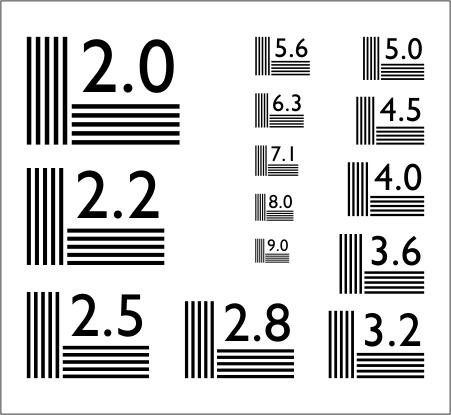
\includegraphics[width=8cm,height=6cm]{resolution_test}
  \caption[caption]{Example Resolution Test Targets (not to scale)\cite{test_chart}}
\end{figure}

\par
Running the laser scanner over the actual resolution test targets above gave us a much clearer indicator of whether or not our scanner was actually able to resolve up to 12.83 $\frac{lines}{mm}$. We ran the laser directly over the five lines in each resolution test target while reading in the values, starting with the lowest resolution.

\pgfplotstableread{scan_1.6.txt}
  \dataone
\begin{figure}[H]
  \centering
  \begin{tikzpicture}
    \begin{axis}[
      xlabel={$time$},
      ylabel={$relative\ intensity$},
      xticklabels={,,},
      yticklabels={,,}]
      \addplot[mark=none] table from \dataone;
    \end{axis}
  \end{tikzpicture}
  \caption[caption]{Scan of 1.6 $\frac{lines}{mm}$ resolution test target}
\end{figure}

\par
In figure 4, five discrete dips in the relative intensity read by the Arduino are visible as the laser passes over the 1.6 $\frac{lines}{mm}$ resolution test target. Each dip is distinguishable and corresponds to a line on the resolution test target. As long as each dip in the relative intensity is discrete for that test, we will consider it a resolvable resolution.

\pgfplotstableread{scan_1.8.txt}
  \datatwo
\begin{figure}[H]
  \centering
  \begin{tikzpicture}
    \begin{axis}[
      xlabel={$time$},
      ylabel={$relative\ intensity$},
      xticklabels={,,},
      yticklabels={,,}]
      \addplot[mark=none] table from \datatwo;
    \end{axis}
  \end{tikzpicture}
  \caption[caption]{Scan of 1.8 $\frac{lines}{mm}$ resolution test target}
\end{figure}

\pgfplotstableread{scan_2.0.txt}
  \datathree
\begin{figure}[H]
  \centering
  \begin{tikzpicture}
    \begin{axis}[
      xlabel={$time$},
      ylabel={$relative\ intensity$},
      xticklabels={,,},
      yticklabels={,,}]
      \addplot[mark=none] table from \datathree;
    \end{axis}
  \end{tikzpicture}
  \caption[caption]{Scan of 2.0 $\frac{lines}{mm}$ resolution test target}
\end{figure}

\pgfplotstableread{scan_2.2.txt}
  \datathree
\begin{figure}[H]
  \centering
  \begin{tikzpicture}
    \begin{axis}[
      xlabel={$time$},
      ylabel={$relative\ intensity$},
      xticklabels={,,},
      yticklabels={,,}]
      \addplot[mark=none] table from \datathree;
    \end{axis}
  \end{tikzpicture}
  \caption[caption]{Scan of 2.2 $\frac{lines}{mm}$ resolution test target}
\end{figure}

\pgfplotstableread{scan_2.5.txt}
  \datathree
\begin{figure}[H]
  \centering
  \begin{tikzpicture}
    \begin{axis}[
      xlabel={$time$},
      ylabel={$relative\ intensity$},
      xticklabels={,,},
      yticklabels={,,}]
      \addplot[mark=none] table from \datathree;
    \end{axis}
  \end{tikzpicture}
  \caption[caption]{Scan of 2.5 $\frac{lines}{mm}$ resolution test target}
\end{figure}

\pgfplotstableread{scan_2.8.txt}
  \datathree
\begin{figure}[H]
  \centering
  \begin{tikzpicture}
    \begin{axis}[
      xlabel={$time$},
      ylabel={$relative\ intensity$},
      xticklabels={,,},
      yticklabels={,,}]
      \addplot[mark=none] table from \datathree;
    \end{axis}
  \end{tikzpicture}
  \caption[caption]{Scan of 2.8 $\frac{lines}{mm}$ resolution test target}
\end{figure}

\pgfplotstableread{scan_3.2.txt}
  \datathree
\begin{figure}[H]
  \centering
  \begin{tikzpicture}
    \begin{axis}[
      xlabel={$time$},
      ylabel={$relative\ intensity$},
      xticklabels={,,},
      yticklabels={,,}]
      \addplot[mark=none] table from \datathree;
    \end{axis}
  \end{tikzpicture}
  \caption[caption]{Scan of 3.2 $\frac{lines}{mm}$ resolution test target}
\end{figure}

\pgfplotstableread{scan_4.0.txt}
  \datathree
\begin{figure}[H]
  \centering
  \begin{tikzpicture}
    \begin{axis}[
      xlabel={$time$},
      ylabel={$relative\ intensity$},
      xticklabels={,,},
      yticklabels={,,}]
      \addplot[mark=none] table from \datathree;
    \end{axis}
  \end{tikzpicture}
  \caption[caption]{Scan of 4.0 $\frac{lines}{mm}$ resolution test target}
\end{figure}

\section{Analysis}
\par
Figures 5 to 11 show our scan data as we increase the resolution of our test target. As the resolution increases, the variance in relative intensity between the lines and the space between them becomes muddled. It is possible to see five discrete dips only up to 3.2 $\frac{lines}{mm}$. At 4.0 $\frac{lines}{mm}$, it is no longer possible to discern five discrete dips in the relative intensity detected. Our testable scanner resolution limit, therefore, is 3.2 $\frac{lines}{mm}$.
\par
We could likely improve our resolution by focusing the laser to a smaller point. Due to human error, our lenses were probably not optimally aligned and we did not focus the laser to a small enough point. Additionally, we could improve the scanner by reducing the radius of the axle pulling the sample across the laser, which would reduce the step distance and increase the precision.

\section{Experimental Results for 2 Dimensional Scans}
\par
For two dimensional scans, instead of running the sample in one direction under the laser, we oscillated it back and forth in the $x$ direction while shifting it in the $y$ direction. This allowed us to produce a two-dimensional image of the lines on the resolution test target by mapping the values onto a 2D grid.

\begin{figure}[H]
  \centering
  
\includegraphics[width=8cm,height=6cm]{2d_scan_1}
  \caption[caption]{Two Dimensional Scan of the 1.6 $\frac{lines}{mm}$ Test Target}
\end{figure}

\par
For demonstration purposes, we used a lower resolution test target so that we could produce a discernible image. We scaled the voltage received by the Arduino to a greyscale value and plotted it based on the motor's position to create the image. However, the motor would slightly drift after each oscillation, creating the slanted lines visible in the scan above.

\begin{figure}[H]
  \centering
  
\includegraphics[width=8cm,height=6cm]{2d_scan_2}
  \caption[caption]{Two Dimensional Scan with Drift Adjustment}
\end{figure}

\par
We were able to reduce some of the slanting by manually accounting for the drift in the motors. Some noise is visible in both of the scans due to the flexing of test target during scanning since it was printed on standard printer paper.

\newpage

\begin{thebibliography}{9}

  \bibitem{amazon}
  Amazon.
  \textit{USPRO 28BYJ Stepper Motors + ULN2003 Driver Board}
  \texttt{https://www.amazon.com/USPRO-Stepper-28BYJ-48-4-Phase-ULN2003/}
  \texttt{dp/B00JB22IQC}

  \bibitem{arduino}
  Arduino.
  \textit{References and Guides}\newline
  \texttt{https://www.arduino.cc/}

  \bibitem{github}
  GitHub.
  \textit{im-firing-my-lazer repository}
  Alvin Lin, 2016\newline
  \texttt{https://www.github.com/omgimanerd/im-firing-my-lazer}

  \bibitem{laser_scanning_paper}
  Peter Axelsson.
  \textit{Processing of laser scanner data - algorithms and applications}.
  Department of Geodesy and Photogrammetry, Royal Institute of Technology, Stockholm, Sweden, 1998.\newline
  \texttt{http://warnercnr.colostate.edu/~lefsky/isprs/1133.pdf}

  \bibitem{thinkquest}
  ThinkQuest.
  \textit{Lenses and optics}
  American Physical Society, 2006\newline
  \texttt{http://www.physicscentral.com/experiment/physicsquest/past/upload/}
  \texttt{pq06-Extension4.pdf}

  \bibitem{test_chart}
  USAF Test Chart
  \textit{High Definition Test Slides}
  Pyser-SGI\newline
  \texttt{http://www.pyser-sgi.com/graticules/graticules-news/usaf-test-chart-}
  \texttt{gets-higher-definition}

\end{thebibliography}

\newpage

\appendix
\section{Appendix A: Code Resources}

\subsection{Arduino code for 1 dimensional scanning}
\begin{lstlisting}[language=C]
#include <Stepper.h>

// Globals
#define BAUDRATE 9600
#define NUM_POLLS 10

#define SCAN_SPEED 60
#define SCAN_STEPS 700
#define SCAN_INTERVAL 1

Stepper motor(512, 8, 10, 9, 11);

void setup() {
  Serial.begin(BAUDRATE);
  for (int i = 8; i < 12; ++i) {
    pinMode(i, OUTPUT);
  }
  motor.setSpeed(SCAN_SPEED);
}

void loop() {
  String data = Serial.readString();
  float value_sum = 0;
  Serial.println(data);
  if (data == "begin") {
    Serial.println("{ \"type\": \"1d\" }");
    for (int i = 0; i < SCAN_STEPS; ++i) {
      value_sum = 0;
      for (int j = 0; j < NUM_POLLS; ++j) {
        value_sum += analogRead(A0);
      }
      Serial.println(value_sum / 10.0);
      motor.step(SCAN_INTERVAL);
    }
    Serial.println("end");
    motor.step(-SCAN_INTERVAL * SCAN_STEPS);
  }
}
\end{lstlisting}

\subsection{Arduino code for 2 dimensional scanning}
\begin{lstlisting}[language=C]
#include <Stepper.h>

// Globals
#define BAUDRATE 9600
#define NUM_POLLS 10

#define SCAN_SPEED 40
#define X_SCAN_STEPS 20
#define X_SCAN_INTERVAL 50
#define Y_SCAN_STEPS 150
#define Y_SCAN_INTERVAL 5

// The motor drifts some amount every y-iteration. This constant fights against that.
#define DRIFT_CONSTANT -50

Stepper x_motor(512, 4, 6, 5, 7);
Stepper y_motor(512, 8, 10, 9, 11);

void setup() {
  Serial.begin(BAUDRATE);
  for (int i = 4; i < 12; ++i) {
    pinMode(i, OUTPUT);
  }
  x_motor.setSpeed(SCAN_SPEED);
  y_motor.setSpeed(SCAN_SPEED);
}

void loop() {
  String data = Serial.readString();
  float value_sum = 0;
  Serial.println(data);
  if (data == "begin") {
    Serial.print("{ \"type\": \"2d\", \"width\": ");
    Serial.print(Y_SCAN_STEPS);
    Serial.print(", \"height\": ");
    Serial.print(X_SCAN_STEPS);
    Serial.print(" }\n");
    for (int x = 0; x < X_SCAN_STEPS; ++x) {
      for (int y = 0; y < Y_SCAN_STEPS; ++y) {
        value_sum = 0;
        for (int i = 0; i < NUM_POLLS; ++i) {
          value_sum += analogRead(A0);
          delay(2);
        }
        Serial.println(value_sum / 10.0);
        y_motor.step(Y_SCAN_INTERVAL);
      }
      y_motor.step(-(Y_SCAN_INTERVAL * Y_SCAN_STEPS - DRIFT_CONSTANT));
      x_motor.step(X_SCAN_INTERVAL);
    }
    Serial.println("end");
    x_motor.step(-X_SCAN_INTERVAL * X_SCAN_STEPS);
    y_motor.step(-Y_SCAN_INTERVAL * Y_SCAN_STEPS);
  }
}
\end{lstlisting}

\subsection{Python code to visualize the stored data}
\begin{lstlisting}[language=Python]
#!/usr/bin/python

from matplotlib import pyplot
from PIL import Image

import argparse
import json
import numpy as np

class Visualizer:

    @staticmethod
    def visualize(data):
        visualize_functions = {
            "1d": Visualizer.visualize_1d,
            "2d": Visualizer.visualize_2d
        }
        visualize_functions[data["type"]](data)

    @staticmethod
    def visualize_1d(data):
        figure = pyplot.figure()
        figure.suptitle("Intensity vs motor ticks")
        values = data["values"]
        pyplot.plot(range(len(values)), values)
        pyplot.xlabel("Motor ticks")
        pyplot.ylabel("Relative Intensity")
        pyplot.grid()
        pyplot.show()

    @staticmethod
    def _linear_scale(x, a1, a2, b1, b2):
        return ((x - a1) * (b2 - b1) / (a2 - a1)) + b1

    @staticmethod
    def _to_pil_data(values):
        low, high = min(values), max(values)
        return map(lambda x: Visualizer._linear_scale(x, low, high, 0, 255),
                   values)

    @staticmethod
    def visualize_2d(data):
        width = data["width"]
        height = data["height"]
        image = Image.new("1", (width, height))
        image.putdata(Visualizer._to_pil_data(data["values"]))
        image = image.resize((width * 8, height * 8), Image.ANTIALIAS)
        image.show()

if __name__ == "__main__":
    parser = argparse.ArgumentParser()
    parser.add_argument("filename", help="The JSON file containing the data")
    args = parser.parse_args()
    with open(args.filename) as data_file:
        Visualizer.visualize(json.loads(data_file.read().strip()))
\end{lstlisting}

\subsection{Python code to read the data from the serial port}
\begin{lstlisting}
#!/usr/bin/python

from lib.visualizer import Visualizer

import argparse
import json
import serial
import sys
import time

class Scanner():

    BAUDRATE = 9600
    AMPLIFYING_FACTOR = 3

    def __init__(self, serial):
        self.serial = serial

    @staticmethod
    def create(location):
        return Scanner(serial.Serial(location, Scanner.BAUDRATE))

    def read(self):
        return self.serial.readline().strip()

    def write(self, data):
        self.serial.write(data)

    def read_laser_info(self):
        data = {}
        values = []
        read = None
        while read != "begin":
            self.write("begin")
            read = self.read()
        while True:
            read = self.read()
            if read == "end":
                break
            print "Received %s" % read
            try:
                values.append(float(read) * 2)
            except ValueError:
                try:
                    data.update(json.loads(read))
                except:
                    continue
        data.update({
            "values": values
        })
        return data

if __name__ == "__main__":
    argparser = argparse.ArgumentParser()
    argparser.add_argument("serial_port", help="The serial port to read from")
    args = argparser.parse_args()

    print "Generating a scanner data visualization..."
    scanner = Scanner.create(args.serial_port)
    data = scanner.read_laser_info()

    Visualizer.visualize(data)

    print "Type a filename to save, otherwise press enter to exit..."
    filename = raw_input()
    if filename != "":
        with open("data/%s.json" % filename, "w") as f:
            f.write(json.dumps(data))
\end{lstlisting}

\end{document}
